\lecture_date{10/11/2026}
\chapter{Lecture 09}
Lecture 08 covered the reverse-mode steps. This lecture extends them to multiple outputs and introduces forward-mode AD.

\begin{example}[RMAD with two outputs and constants]
At $(x_1,x_2)=(1,1)$, find the gradients of
\[
 F(x_1,x_2)=\begin{bmatrix}f_1\\f_2\end{bmatrix}
 =\begin{bmatrix}2x_1/x_2\\x_1x_2+5\end{bmatrix},\qquad x_2\ne0.
\]
\end{example}
Using the method from Lecture 08, set $u=x_2^{-1}$ and $v=x_1x_2$. Then $f_1=2x_1u$ and $f_2=v+5$.
\begin{center}
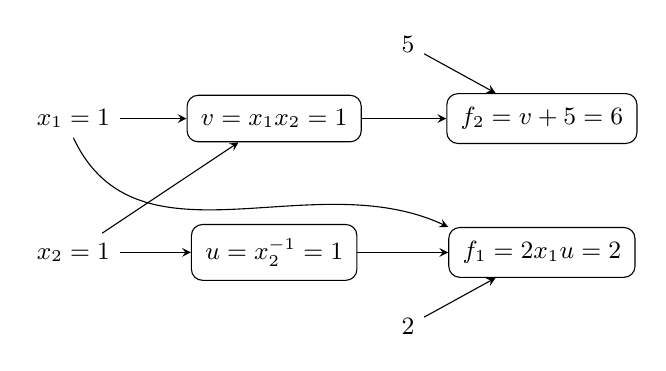
\begin{tikzpicture}[scale=.85,>=stealth,every node/.style={font=\small},op/.style={draw,rounded corners,align=center,inner sep=5pt}]
\node (x1) at (0,1) {$x_1=1$};
\node (x2) at (0,-1) {$x_2=1$};
\node[op] (u) at (3,-1) {$u=x_2^{-1}=1$};
\node[op] (v) at (3,1) {$v=x_1x_2=1$};
\node[op] (f1) at (7,-1) {$f_1=2x_1u=2$};
\node[op] (f2) at (7,1) {$f_2=v+5=6$};
\node (c2) at (5,-2.1) {$2$};
\node (c5) at (5,2.1) {$5$};
\draw[->] (x1)--(v); \draw[->] (x2)--(v);
\draw[->] (x2)--(u); \draw[->] (u)--(f1);
\draw[->] (x1.south) to[out=-65,in=155] (f1.north west);
\draw[->] (v)--(f2); \draw[->] (c2)--(f1); \draw[->] (c5)--(f2);
\end{tikzpicture}


\end{center}
The required local derivatives, evaluated at $(1,1)$, are
\[
 u_{x_2}=-x_2^{-2}=-1,\quad v_{x_1}=x_2=1,\quad v_{x_2}=x_1=1,
\]
\[
 \left.\frac{\partial f_1}{\partial x_1}\right|_u=2u=2,
 \qquad \frac{\partial f_1}{\partial u}=2x_1=2,
 \qquad \frac{\partial f_2}{\partial v}=1.
\]
Constants affect the calculation, but we do not differentiate with respect to the fixed numbers $2$ and $5$.

\subsubsection*{Select an output, then accumulate backward}
For $f_1$, seed $(\bar f_1,\bar f_2)=(1,0)$. Thus
\[
 \bar u=2,\quad \bar v=0,\quad
 \bar x_1=1\cdot2+0\cdot1=2,\quad
 \bar x_2=2(-1)+0\cdot1=-2.
\]
Reset the adjoints. For $f_2$, seed $(\bar f_1,\bar f_2)=(0,1)$. Then
\[
 \bar u=0,\quad \bar v=1,\quad
 \bar x_1=0\cdot2+1\cdot1=1,\quad
 \bar x_2=0(-1)+1\cdot1=1.
\]
Hence $\boxed{\nabla f_1(1,1)=(2,-2)^T,\quad\nabla f_2(1,1)=(1,1)^T.}$


\clearpage
\section{Forward-mode automatic differentiation}
In forward mode, derivatives travel from the inputs towards the outputs, in the same direction as the function values.

\subsection{The seed variable and dot notation}
The lecturer introduces a seed variable $s$ and writes
\[
 \dot x_i=\frac{dx_i}{ds},\qquad \dot u=\frac{du}{ds}.
\]
To calculate the derivative with respect to $x_1$, set $s=x_1$: then $\dot x_1=1$ and the other input derivatives are $0$. For example, with three inputs,
\[
\begin{array}{c|ccc}
 &\dot x_1&\dot x_2&\dot x_3\\\hline
s=x_1&1&0&0\\
s=x_2&0&1&0\\
s=x_3&0&0&1
\end{array}
\]
\textbf{Only the dot values change between passes.} The input point and the ordinary node values stay fixed. A constant has dot derivative $0$.

\subsection{Steps of forward-mode AD}
\begin{enumerate}
\item Generate the computational graph.
\item Name the intermediate nodes.
\item Calculate their values at the given input point.
\item Write each node's derivative with respect to the seed variable $s$.
\item Set $s=x_i$, so $\dot x_i=1$ and the other input dot values are $0$.
\item Accumulate the derivatives forward, then repeat steps 5--6 for each remaining input.
\end{enumerate}
One pass gives the derivative of every output with respect to the selected input. Thus we need one pass per input to obtain all the gradient components.

\subsubsection*{Rules used in the examples}
Apply the ordinary sum, product and chain rules:
\[
\begin{aligned}
 u=ab &\quad\Longrightarrow\quad \dot u=\dot a\,b+a\dot b,\\
 u=a+b &\quad\Longrightarrow\quad \dot u=\dot a+\dot b,\\
 u=a^2 &\quad\Longrightarrow\quad \dot u=2a\dot a,\\
 u=\sin a &\quad\Longrightarrow\quad \dot u=(\cos a)\dot a.
\end{aligned}
\]
For example, $u=x_1x_2$ gives
\[
\frac{du}{ds}=\frac{dx_1}{ds}x_2+x_1\frac{dx_2}{ds}
=\dot x_1x_2+x_1\dot x_2.
\]
Write these formulas once beside the graph; show the calculations for each seed in a table below it.

\clearpage
\begin{example}[A shared product in forward mode]
Find the gradient of
\[
 f(x_1,x_2,x_3)=3x_1x_2\sin(x_1x_2+x_3^2)
 \quad\text{at }\left(\frac\pi2,1,0\right).
\]
\end{example}
Set $u_1=x_1x_2$, $u_2=x_3^2$, $v=u_1+u_2$, $w=\sin v$, and $f=3u_1w$. Reuse the same $u_1$ in both places.
\begin{center}
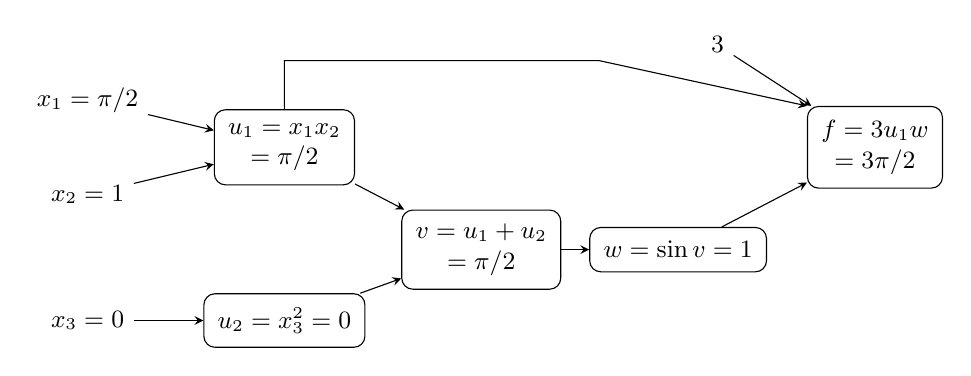
\begin{tikzpicture}[>=stealth,every node/.style={font=\small},op/.style={draw,rounded corners,align=center,inner sep=5pt}]
\node (x1) at (0,1.4) {$x_1=\pi/2$};
\node (x2) at (0,.2) {$x_2=1$};
\node (x3) at (0,-1.4) {$x_3=0$};
\node[op] (u1) at (2.5,.8) {$u_1=x_1x_2$\\$=\pi/2$};
\node[op] (u2) at (2.5,-1.4) {$u_2=x_3^2=0$};
\node[op] (v) at (5,-.5) {$v=u_1+u_2$\\$=\pi/2$};
\node[op] (w) at (7.5,-.5) {$w=\sin v=1$};
\node[op] (f) at (10,.8) {$f=3u_1w$\\$=3\pi/2$};
\node (c) at (8,2.1) {$3$};
\draw[->] (x1)--(u1); \draw[->] (x2)--(u1); \draw[->] (x3)--(u2);
\draw[->] (u1)--(v); \draw[->] (u2)--(v); \draw[->] (v)--(w); \draw[->] (w)--(f);
\draw[->] (u1.north)--(2.5,1.9)--(6.5,1.9)--(f.north west); \draw[->] (c)--(f);
\end{tikzpicture}
\end{center}
The formulas used in every seeded sweep are
\begin{align*}
 \dot u_1&=\dot x_1x_2+x_1\dot x_2,&
 \dot u_2&=2x_3\dot x_3,\\
 \dot v&=\dot u_1+\dot u_2,&
 \dot w&=(\cos v)\dot v,\\
 \dot f&=3(\dot u_1w+u_1\dot w).
\end{align*}
At the given point, $x_3=0$ and $\cos v=\cos(\pi/2)=0$. Consequently $\dot u_2=\dot w=0$ for all three coordinate seeds.
\begin{center}
\renewcommand{\arraystretch}{1.35}
\begin{tabular}{lccc}
\toprule
Quantity & $s=x_1$ & $s=x_2$ & $s=x_3$\\
\midrule
$(\dot x_1,\dot x_2,\dot x_3)$ & $(1,0,0)$ & $(0,1,0)$ & $(0,0,1)$\\
$\dot u_1$ & $1\cdot1+(\pi/2)0=1$ & $0\cdot1+(\pi/2)1=\pi/2$ & $0$\\
$\dot u_2$ & $0$ & $0$ & $2\cdot0\cdot1=0$\\
$\dot v$ & $1$ & $\pi/2$ & $0$\\
$\dot w$ & $0$ & $0$ & $0$\\
$\dot f$ & $3$ & $3\pi/2$ & $0$\\
\bottomrule
\end{tabular}
\end{center}
Thus
\[
 \boxed{\nabla f\left(\frac\pi2,1,0\right)=\begin{bmatrix}3\\3\pi/2\\0\end{bmatrix}.}
\]
For example, the first sweep ends with $\dot f=3(1\cdot1+(\pi/2)0)=3$. It gives only $\partial f/\partial x_1$, not the entire gradient. Three coordinate sweeps give its three components.


\clearpage
\begin{example}[Several outputs from shared intermediate nodes]
Find the three gradients at $(1,1)$:
\[
 f_1=x_1^2x_2^3,\qquad
 f_2=x_1^2\sin(x_2^3),\qquad
 f_3=x_1^2+x_2^3.
\]
\end{example}
Use $u_1=x_1^2$, $u_2=x_2^3$, and $v=\sin u_2$. Then
\[
 (f_1,f_2,f_3)=(u_1u_2,u_1v,u_1+u_2).
\]
\begin{center}
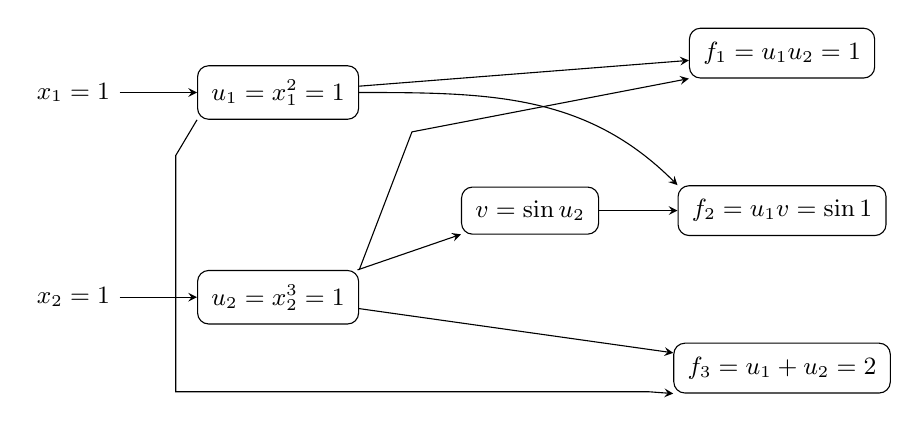
\begin{tikzpicture}[>=stealth,every node/.style={font=\small},op/.style={draw,rounded corners,align=center,inner sep=5pt}]
\node (x1) at (0,1.3) {$x_1=1$};
\node (x2) at (0,-1.3) {$x_2=1$};
\node[op] (u1) at (2.6,1.3) {$u_1=x_1^2=1$};
\node[op] (u2) at (2.6,-1.3) {$u_2=x_2^3=1$};
\node[op] (v) at (5.8,-.2) {$v=\sin u_2$};
\node[op] (f1) at (9,1.8) {$f_1=u_1u_2=1$};
\node[op] (f2) at (9,-.2) {$f_2=u_1v=\sin1$};
\node[op] (f3) at (9,-2.2) {$f_3=u_1+u_2=2$};
\draw[->] (x1)--(u1); \draw[->] (x2)--(u2);
\draw[->] (u1)--(f1); \draw[->] (u2.north east)--(4.3,.8)--(f1.south west);
\draw[->] (u2)--(v); \draw[->] (v)--(f2); \draw[->] (u1.east) to[out=0,in=135] (f2.north west);
\draw[->] (u2)--(f3); \draw[->] (u1.south west) --(1.3,.5)--(1.3,-2.5)--(7.3,-2.5)--(f3.south west);
\end{tikzpicture}

\small Crossings without a node do not indicate a dependency.
\end{center}
The propagation rules are
\begin{align*}
 \dot u_1&=2x_1\dot x_1,& \dot u_2&=3x_2^2\dot x_2,&
 \dot v&=(\cos u_2)\dot u_2,\\
 \dot f_1&=\dot u_1u_2+u_1\dot u_2,&
 \dot f_2&=\dot u_1v+u_1\dot v,&
 \dot f_3&=\dot u_1+\dot u_2.
\end{align*}
\begin{center}
\renewcommand{\arraystretch}{1.3}
\begin{tabular}{lcc}
\toprule
Quantity & $s=x_1$: $(\dot x_1,\dot x_2)=(1,0)$ & $s=x_2$: $(0,1)$\\
\midrule
$\dot u_1$ & $2$ & $0$\\
$\dot u_2$ & $0$ & $3$\\
$\dot v$ & $0$ & $3\cos1$\\
$\dot f_1$ & $2\cdot1+1\cdot0=2$ & $0\cdot1+1\cdot3=3$\\
$\dot f_2$ & $2\sin1+1\cdot0=2\sin1$ & $0\sin1+1(3\cos1)=3\cos1$\\
$\dot f_3$ & $2+0=2$ & $0+3=3$\\
\bottomrule
\end{tabular}
\end{center}
Each pass gives one component of each of the three gradients. Collecting the results,
\[
 \boxed{\nabla f_1(1,1)=\begin{bmatrix}2\\3\end{bmatrix},\quad
 \nabla f_2(1,1)=\begin{bmatrix}2\sin1\\3\cos1\end{bmatrix},\quad
 \nabla f_3(1,1)=\begin{bmatrix}2\\3\end{bmatrix}.}
\]
Two forward passes give all three gradients; reverse mode would need three reverse passes. Trigonometric arguments are in radians.

\clearpage
\begin{remark}[A correction to the quotient example]
The lecturer initially used $q=x_1^2/x_2^3$, then replaced it with $x_1^2\sin(x_2^3)$. The example on the previous page follows the final version. However, the original quotient also works in forward mode at $(1,1)$.

Set $u_1=x_1^2$, $u_2=x_2^3$, $v=1/u_2$, and $q=u_1v$. The important rule is
\[
 \boxed{\dot v=-\frac{\dot u_2}{u_2^2}.}
\]
At $(1,1)$, $u_2=1$. If $\dot u_2=0$, then $\dot v=0$; there is no division by zero. The denominator uses the \emph{value} $u_2$, not its dot derivative.
\begin{center}
\renewcommand{\arraystretch}{1.3}
\begin{tabular}{lcc}
\toprule
 & $s=x_1$ & $s=x_2$\\
\midrule
$(\dot u_1,\dot u_2)$ & $(2,0)$ & $(0,3)$\\
$\dot v=-\dot u_2/u_2^2$ & $0$ & $-3$\\
$\dot q=\dot u_1v+u_1\dot v$ & $2$ & $-3$\\
\bottomrule
\end{tabular}
\end{center}
Hence $\nabla q(1,1)=(2,-3)^T$. The actual restriction is $x_2\ne0$: at $x_2=0$ the function is undefined, regardless of the AD mode. Zero dot values alone are not an instability of forward mode.
\end{remark}

\section{Forward mode versus reverse mode}
For the one-input-at-a-time and one-output-at-a-time calculations used in class:

\begin{center}
\renewcommand{\arraystretch}{1.35}
\begin{tabular}{
  >{\raggedright\arraybackslash}p{2.5cm}
  >{\raggedright\arraybackslash}p{4.8cm}
  >{\raggedright\arraybackslash}p{4.8cm}
}
\toprule
 & Forward mode & Reverse mode\\
\midrule
Direction
 & Derivatives accumulate from inputs to outputs
 & Derivatives accumulate from outputs to inputs\\
One pass gives
 & One component of every output's gradient
 & The whole gradient of one selected output\\
Repeats needed
 & One forward pass per input
 & One reverse pass per output, after forward evaluation\\
Most useful when
 & Inputs are few, outputs are many
 & Inputs are many, outputs are few\\
\bottomrule
\end{tabular}
\end{center}

Reverse mode first evaluates the graph and stores intermediate information needed for the backward passes, creating a memory overhead. For multiple outputs, reset the adjoints between reverse passes; the stored forward values can be reused. Forward mode carries values and dot derivatives forward and usually requires less storage, though it still needs working memory.

A model with many parameters and one scalar loss is therefore well suited to reverse mode: one reverse pass gives the whole gradient. In this lecture's example with two inputs and three outputs, forward mode needs two passes, whereas reverse mode needs three reverse passes after evaluating the graph.